% !TeX spellcheck = de_DE
\documentclass[
	oneside,  % falls doppelseitiger Druck gewünscht, "oneside" durch "twoside" ersetzen
	ngerman, 
	final, 
	11pt, 
	a4paper, 
	1.1headlines, 
	headinclude=false, 
	footinclude=false, 
	mpinclude=false, 
	pagesize, 
	onecolumn, 
	titlepage, 
	parskip=half, 
	headsepline, 
	chapterprefix=false, 
	version=first, 
	listof=totoc, 
	bibliography=totoc, 
	toc=graduated, 
	fleqn
]{scrbook}

%%%%%%%%%%% Verwendete Pakete %%%%%%%%%%%
\usepackage[T1]{fontenc}
\usepackage[utf8]{inputenc}
\usepackage{babel}
\usepackage{hyperref}
\usepackage[table]{xcolor}
\usepackage{booktabs}
\hypersetup{
	colorlinks=true,
	linkcolor=black,
	urlcolor=black,
	linktoc=all,
	citecolor=black
}
\usepackage{float}
\usepackage{graphicx}
\usepackage{textpos} 
\usepackage{tocloft}
\usepackage{lipsum}
\usepackage{color}
\usepackage[onehalfspacing]{setspace}
\usepackage{acronym}
\usepackage{multicol}
\usepackage{url}

% Einbindung und Konfiguration von nomencl für Nomenklaturen
\usepackage{nomencl}

\renewcommand{\nomname}{Abkürzungsverzeichnis}

\providecommand{\printnomenclature}{\printglossary}
\providecommand{\makenomenclature}{\makeglossary}
\makenomenclature

% Einbindung und Konfiguration von listings für Quellcode-Listings
\usepackage{listings}

\renewcommand\lstlistlistingname{Quellcodeverzeichnis}
\renewcommand{\lstlistingname}{Quellcode}

\lstset{language=OCL} 

\definecolor{default-lst-background}{RGB}{242,242,242}
\definecolor{default-lst-keyword}{RGB}{94,20,64}
\definecolor{default-lst-string}{RGB}{15,26,250}
\definecolor{default-lst-comment}{RGB}{31,97,46}

\definecolor{eclipse-java-background}{RGB}{235,235,235}
\definecolor{eclipse-java-keyword}{RGB}{127,0,85}
\definecolor{eclipse-java-string}{RGB}{42,0,255}
\definecolor{eclipse-java-comment}{RGB}{63,127,95}
\definecolor{eclipse-java-annotation}{RGB}{127,159,191}

\lstset{
	basicstyle={\footnotesize\fontfamily{pcr}\selectfont},
	backgroundcolor=\color{default-lst-background},
	keywordstyle=\color{default-lst-keyword}\bfseries,	
	stringstyle=\color{default-lst-string},
	commentstyle=\color{default-lst-comment}\itshape,
	frame=single,
	numbers=left,
	captionpos=b,
	showstringspaces=false,
	breaklines=true,
	tabsize=2
}

%% Listing-Style für Java, der das Syntax Highlighting wie in Eclipse vornimmt
\lstdefinestyle{eclipse-java}{	
	backgroundcolor=\color{eclipse-java-background},
	keywordstyle={\color{eclipse-java-keyword}\bfseries},
	stringstyle={\color{eclipse-java-string}},
	commentstyle={\color{eclipse-java-comment}},		
	moredelim={[il][\textcolor{eclipse-java-annotation}]{\%}},
	moredelim={[is][\textcolor{eclipse-java-annotation}]{\%\%}{\%\%}}
}

%%%%%%%%%%% Weitere Konfigurationen %%%%%%%%%%%
% Schachtelungstiefe
\setcounter{secnumdepth}{3}
\setcounter{tocdepth}{3}

% Schriftart
\makeatletter
\setkomafont{disposition}{\normalcolor\bfseries}
\makeatother

% Balkenfarbe Titelseite
\definecolor{titlepage-rule-color}{RGB}{194,191,194}

%%%%%%%%%%% Angaben zur Arbeit und Autorinnenschaft %%%%%%%%%%%
% Angaben zu Ihrer Arbeit. Bitte ersetzen Sie die Werte der Makros durch die passenden.
%% Art der Arbeit. Gültige Werte: "Projektarbeit", "Bachelorthesis", "Masterseminar", "F\&E-Arbeit", "Masterthesis".
\newcommand*{\fhdopaperkind}{Bachelor Thesis}
%% Titel
\newcommand*{\fhdopapertitle}{Konzeption und Implementierung einer Model-to-Model Transformation zur Überführung unterspezifierter Domänenmodelle in Micoservices}
%% optionaler Untertitel, der etwas länger als der Titel sein kann
\newcommand*{\fhdopapersubtitle}{}
%% Datum der Abgabe im Format DD.MM.YYYY
\newcommand*{\fhdopaperdate}{26.08.2018}
%% erste Betreuerin
\newcommand*{\fhdopaperfirstsupervisor}{Prof. Dr. Sabine Sachweh} 
%% zweite Betreuerin inklusive Abschluss, also z. B. "B.Sc." oder "M.Sc."
\newcommand*{\fhdopapersecondsupervisor}{Florian Rademacher, M. Sc.}

% Angaben zu Ihnen als Autorin. Bitte ersetzen Sie die Werte der Makros durch die passenden.
%% vollständiger Name
\newcommand*{\fhdopaperauthor}{Till Paplowski}
%% Geburtstag
\newcommand*{\fhdopaperbirthday}{09.03.1995}
%% Matrikelnummer
\newcommand*{\fhdopaperstudentnumber}{7090903}
%% Studiengang
\newcommand*{\fhdopapermajor}{Software und Systemtechnik}
%% Der durch Ihren Studiengang angestrebte Abschluss. Gültige Werte: "Bachelor", "Master".
\newcommand*{\fhdopaperdegree}{Bachelor of Science} 

\begin{document}
%%%%%%%%%%% Titelseite. Bitte unverändert lassen. %%%%%%%%%%%
\begin{titlepage}
	\begin{textblock}{6.5}(-1,-3)
		\begin{color}{titlepage-rule-color}
			\rule{6.8cm}{33cm}    
		\end{color}
	\end{textblock}

	\begin{textblock}{6.5}(-0.8,1)\textsf{%
		\Large 
		\fhdopaperkind
	}\end{textblock}

	\begin{textblock}{7}(4.5,2)\textsf{%
		\noindent 
		\huge 
		\textbf{\fhdopapertitle}\\[0.3cm] 
		\Large \fhdopapersubtitle\\[0.05cm]
	}\end{textblock}

	\begin{textblock}{6}(4.5,6.5)\textsf{%
		\noindent
		An der Fachhochschule Dortmund\\
		im Fachbereich Informatik\\
		Studiengang \fhdopapermajor{}\\
		erstellte \fhdopaperkind{}\\
		zur Erlangung des akademischen Grades\\
		\fhdopaperdegree{} of Science
	}\end{textblock}

	\begin{textblock}{6.5}(-0.4,10.0)\textsf{%
		\noindent
		von\\
		\fhdopaperauthor{}\\
		geb. am \fhdopaperbirthday\\
		Matr.-Nr. \fhdopaperstudentnumber\\[0.7cm]
		Betreuer:\\
		\hspace*{6mm} \fhdopaperfirstsupervisor{}\\
		\noindent\hspace*{6mm} \fhdopapersecondsupervisor{}\\[0.5cm]
		Dortmund, \fhdopaperdate
	}\end{textblock}
\end{titlepage}
	
\newpage{}

%%%%%%%%%%% Inhalt der Arbeit. Ab hier sind wieder Änderungen erlaubt. %%%%%%%%%%%

% Kurzfassung
\section*{\thispagestyle{empty}Kurzfassung}
\lipsum[1-2]

\newpage{}

% Abstract (= Kurzfassung auf Englisch)		
\section*{\thispagestyle{empty}Abstract}		
\lipsum[1-2]

\newpage{}

% Inhaltsverzeichnis. Bitte unverändert lassen.
%% Römische Nummerierung
\setcounter{page}{1}
\pagenumbering{roman}
\tableofcontents
		
\newpage{}
		
%% Nach Inhaltsverzeichnis wieder arabische Nummerierung mit Neubeginn Nummerierung
\setcounter{page}{1} 
\pagenumbering{arabic}

% Weiter mit dem Inhalt der Arbeit. Ab hier sind wieder Änderungen erlaubt.

	\chapter{Einleitung}
\label{chap:einleitung}


\section{Motivation}

\section{Zielsetzung}

\section{Vorgehensweise}

\chapter{Grundlagen}
\label{chap:theorie}

\section{Modellgetriebene Softwareentwicklung}

\ac{mdsd}

\subsection{Modellierungssprachen}
- Unterscheidung zwischen GPL und DSML hier rein\\

\subsection{Modelltransformation}
\ac{m2m}
\ac{qvt}

\section{UML-Profil für das Domain-driven Design}

\subsection{Domain-driven Design}
\subsection{Eclipse Papyrus und UML-Profile}
\ac{ocl}
\subsection{UML-Profil zu Erstellung von Domänenmodellen}

\section{AjiL Modeling Language}
\subsection{Der Microservice-Architekturstil}
Hier rein erklärung von MSAs, aber auch grob Erkenntnisse aus der PA bezüflich der Verbindbarkeit von DSML und MSA
\subsection{ECore}
\subsection{AjiL}

\chapter{Analyse der Anforderungen an die Transformation} %Nach IREB
In diesem Kapitel werden die Stakeholder an der Transformation (siehe Abschnitt 5.1) und die Problemdomäne (siehe Abschnitt 5.2) betrachtet und verschiedene Arten von Anforderungen (Siehe ABschnitt 5.3) definiert. %Verweise zu Unterkapiteln nicht vergessen
\section{Stakeholder}
Die üblichen Stakeholder für eine Transformation zwischen zwei \ac{dsml}s lassen sich in drei Kategorien ähnlich \cite{DSMLReq}, welche die Stakeholder für \ac{dsl}s beschreibt, einteilen:
\paragraph{Software- und System-Engineers:} Sind verantwortlich für die Entwicklung und Auswahl der Modellierungssprachen, die transformiert werden. Zudem handelt es sich um Entwickler, die die Transformation weiterentwickeln.
\paragraph{Domänenentwickler:} Nutzen \ac{ajil} zur Entwicklung von Modellen oder Quellcode.
\paragraph{Kunden:} Fungieren als Domänenexperten bei dem Entwurf von Domänenmodellen nach \ac{ddd}, die die Problemdomäne des Kunden beschreiben.
\section{Problemdomäne}
Die Problemdomäne, in der die Transformation angewandt wird, ist die Planung und Modellierung von \ac{msa}s. Hierbei soll eine Möglichkeit geboten werden in Zusammenarbeit mit Domänenexperten entworfene \ac{ddd}-\ac{uml} konforme Domänenmodelle in entsprechende \ac{msa} Modelle nach \ac{ajil} zu transformieren.

Es besteht kein Anspruch, dass alle Komponenten des Domänenmodells in ein \ac{msa} Modell übertragen werden, da nicht alle Konzepte von \ac{ddd} Äquivalente in \ac{ajil} haben.
\section{Anforderungen}
In der folgenden Sektion werden die Anforderungen an die Modeltransformation zwischen dem formalen \ac{ddd}-Profil und \ac{ajil} definiert. Gemä"s ISO/IEC/IEEE 24765 \cite{IEEE10} besitzen Anforderungen drei grundlegende Eigenschaften: 
\begin{itemize}
\item Ein Zustand oder Fähigkeit, die von einem Nutzer benötigt wird, um ein Problem zu lösen oder ein Ziel zu erreichen.
\item Ein Zustand oder Fähigkeit, die von einem System oder einer Systemkomponente  erfüllt oder besessen werden muss, um einem Vertrag, Standards, Spezifikationen oder anderen formal auferlegten Dokumenten nachzukommen.
\item Eine dokumentierte Darstellung des Zustandes oder der Fähigkeit, die in (1) oder (2) beschrieben werden. 
\end{itemize}
Hierbei wird zwischen drei Arten von Anforderungen unterschieden: Funktionale Anforderungen, Qualitätsanforderungen und Randbedingungen. Funktionale Anforderungen an die Transformationen beschreiben die eigentlichen Funktionalitäten der Software. Qualitätsanforderungen beschreiben die qualitiativen Eigenschaften der Software, und Randbedingungen geben Einschränkungen an die Lösung in einem technischen und organisatorischen Rahmen vor. \cite{requirementsGrundlagen} Die Verwendung der Begriffe MUSS und SOLLTE ist angelehnt an ihre Verwendung in der 'MASTeR'-Schablonenreihe um die Verbindlichkeit von Anforderungen auszudrücken. Dementsprechend formulieren MUSS-Anfoderungen Funktionalitäten dar die in jedem Fall umgesetzt werden muss. SOLL-Anforderungen stellen durch Stakeholder gewünschte Funktionalitäten dar, welche aber nicht zwingend umgesetzt werden müssen. \cite{schablonen}

Bei der Erstellung der Anforderungen wird davon ausgegangen, dass der Code, der die Transformation ausführt, in eine ausführbares Software integriert ist. Da in dieser Arbeit keine konkreten Technologien zur Umsetzung bestimmt werden, kann es sich bei dem ausführbaren Software je nach Mächtigkeit der Transformationssprache um die selbe Software handeln, die auch die Transformation beinhaltet, oder um eine Software, welche eine seperate Transformationsdatei ausführt.

\subsection{Funktionale Anforderungen}
\textbf{/F.01/} Die Software MUSS aus einem Modell welches unter Anwendung des \ac{DDD}-\ac{uml}-Profils erstellt und validiert wurde, eine \ac{ajil} konforme Datei erzeugen.

\textbf{/F.01.01/} Die Software SOLL den Typen der Output Datei von .uml in eine .ajimlt Datei ändern.

\textbf{/F.02/} Die Software MUSS die einzelnen \ac{ddd} Komponenten gemäß der Tabelle 4.1 in entsprechende \ac{ajil} Komponenten transformieren.

\textbf{/F.03/} Die Software SOLL durch Nutzer Eingaben Ergebnisse aus den in den Unterabschnitten 4.2.4 und 4.2.6 beschriebenen Verfahren validieren.

\textbf{/F.03/} Die Software SOLL einen Modus ohne Nutzer Eingaben bieten.

\subsection{Qualitätsanforderungen}
\textbf{/Q.01/} Die Software SOLL auf einem herkömmlichen Bürorechner (2 GHz, 2 GB Arbeitsspeicher) ausführbar sein.

\textbf{/Q.02/} Die Transformation SOLL in einer einzelnen Transformationsdatei beschrieben werden.

\textbf{/Q.03/} Die Software MUSS nur notwendige Interfaces und Abilities an Microservices modellieren

\textbf{/Q.04/} Die Software SOLL durch Entwickler an Änderungen im \ac{uml}-Profil oder \ac{ajil} anpassbar sein.
\subsection{Randbedingungen}
\textbf{/R.01/} Die Software SOLL aus der Eclipse Entwicklungsumgebung heraus ausführbar sein.

\chapter{Konzept für die Model-to-Model-Transformation}
Im folgenden Kapitel wird konkret beschrieben und grafisch dargestellt wie Elemente des \ac{ddd}-\ac{uml}-Profils in Elemente von \ac{ajil} übersetzt werden. Hierzu werden die Elemente in semantisch zusammenhängende Gruppen eingeteilt.
\section{Dezidierung von Microservices}
In \cite{BuildingMicroServices} bezieht sich Newman direkt auf Evans \ac{ddd}. Hiernach sollen Microservices exakt Bounded Contexts entsprechen. Für diese These gibt es zahlreiche Argumente.

Bei der Konzeptionierung von \ac{msa}s ist eine der zentralen Fragestellungen die nach der Größe einzelner Microservices. Als Anhaltspunkt wird hierzu das von Robert C. Martin definierte Single Responsibility Prinzip angeführt: \cite{BuildingMicroServices} \textit{„Gather together the things that change for the same reasons. Separate those things that change for different reasons.“} \cite{Martin2003} Dies deckt sich mit Evans Definition eines Microservices als ein  Gültigkeitsbereich, in dem lediglich eine gewisse Fachlogik umgesetzt wird und von anderen Logiken abgegrenzt wird \cite{DDDEvans}. 
- Diese Philosophie entspricht
dem Gedanken von \ac{msa}s, da hier ein Team für einen Microservice zuständig ist, der
keine gemeinsame Implementierung mit anderen Services teilt. \cite{MicroServicesVSSOA}. Ein weiterer Grund für die Einteilung anhand von Bounded Contexts ist, dass Bounded
Contexts durch ihre Eigenschaft nur ein innerhalb des Contexts konsistentes Modell zu
verlangen, einem Team ermöglichen ohne genaue Kenntnis der Objekte und Vorgänge
innerhalb anderer Bounded Contexts zu arbeiten. \ac{ddd} \cite{DDDEvans}.
 %umformulieren da aus PA, eventuell noch kurz auf die Unterscheidung der verschiedenen Ideen aus PA hinweisen?
 Auch in ihrer Funktionsweise weisen Bounded Contexts Ähnlichkeiten zu Microservices auf, da sie geregelte Zugriffspunkte auf die in ihnen enthaltenen Entitäten bieten \cite{DDDEvans}, was der Aufgabe von Interfaces von Microservices ähnelt.
 Aus diesen Gründen sollen bei der Transformation Bounded Contexts in einzelne Microservices überführt werden.

Es sollen bei der Transformation eines \texttt{Package} Elements mit dem Stereotyp \texttt{Bounded Context} folgende Maßnahmen ergriffen werden (vgl. Abbildung 4.1): \textbf{1.)} Erzeugung eines \texttt{FunctionalServiceT} Elements mit dem Namen des \texttt{Bounded Context} und dem hinzugefügten Suffix \textit{Service}. \textbf{2.)} Erzeugung eines \texttt{DataModelT} Elements mit dem Namen des \texttt{Bounded Context}, welches \textbf{3.} dem \texttt{FunctionalServiceT} Element als \texttt{domain} zugeordnet wird. Diese Zuordnung ist in \ac{ajil} stets 1 zu 1. \textbf{4.)} Evans beschreibt auch \texttt{Modules} als Konzept, diese haben jedoch die gleiche Funktionsweise wie  \texttt{Packages} in \ac{uml}, außer, dass Elemente in einem \texttt{Module} keine Beziehungen zu Elementen in anderen \texttt{Modules} haben sollen \cite{DDDEvans}. Im \ac{ddd}-Profil existiert für \texttt{Package} Elemente der Stereotyp \texttt{Module}, jedoch ist keine Beschränkung bezüglich der Beziehungen zwischen \texttt{Modules} implementiert. In \ac{ajil} existiert kein äquivalentes Konzept zu \texttt{Packages} oder \texttt{Modules}. Unter der Annahme, dass die Einschränkungen, die Evans für \texttt{Modules} formuliert in der \ac{uml} Modellierung beachtet wird, verhalten sie sich wie \texttt{DataModels} in \ac{ajil}, und eine solche Transformation wäre sinnvoll. Da jedoch zum Zeitpunkt der Erstellung dieser Arbeit lediglich eine 1 zu 1 Beziehung zwischen \texttt{Service} und \texttt{DataModel} möglich ist, werden zunächst \texttt{Packages} mit dem \texttt{Module} Stereotyp nicht transformiert und lediglich eine entsprechende Log Ausgabe erzeugt.
\begin{figure}
\includegraphics[width=\textwidth]{Bilder/boundedcontext_rules_explained.png}
\caption{Transformation von Bounded Contexts}
\end{figure}
\section{Entities, Enumerations, Value Objects und SharedModels}
Vergleiche Abbildung 4.2.:
\textbf{1.)} Sowohl \texttt{ValueObjects}, \texttt{Enumerations} als auch \texttt{Entities} werden in \texttt{EntityT} Elemente aus \ac{ajil} transformiert. \textbf{2.)} Attribute von \texttt{Value Objects} und \texttt{Entities} werden zu dem entsprechenden primitiven Datentyp in \ac{ajil}. Hierbei ist zu beachten, dass \ac{ddd} Modelle bewusst unterspezifiziert werden können (vgl. Abschnitt 2.2.1). Da es in \ac{ajil} nicht möglich ist ein Attribut ohne Datentypen zu erzeugen, wird in diesem Fall ein \texttt{StringT} Element erzeugt. Darüber hinaus ist es durch Zusammenarbeit mit den Entwicklern von \ac{ajil} auch in \ac{ajil} möglich komplexe Datentypen wie beispielsweise andere \texttt{EntityT} Elemente als Attribut zu verwenden. In diesem Fall soll ein Attribut einer \ac{uml} \texttt{Entity} auch die entsprechende \ac{ajil} \texttt{EntityT} ein  Attribut vom Typ \texttt{EntityT} mit dem gleichen Namen wie die referenzierte \texttt{Entity} erhalten. Dieses Attribut enthält jedoch aufgrund von Limitierung in \ac{ajil} keinen echten Zeiger auf das referenzierte \texttt{EntityT} Element.

\textbf{3.)} Während in \ac{ddd} Operationen an \texttt{Entities} nicht ausgeschlossen werden, und im Fall von \texttt{Value Objects} sogar Teil des Konzepts sind, verfügt \texttt{EntityT} in \ac{ajil}  über keine Operationen. Hier tritt ein Informationsverlust auf. Aus dem gleichen Grund werden \texttt{Specs}, welche sich nur durch ihre Validierungsoperationen definieren, nicht in \ac{ajil} überführt (\textbf{4}), sondern in der Logging-Datei der Transformation ausgegeben. \textbf{5.)} Die \texttt{EnumerationLiterals} von \texttt{Enumerations} werden standardmäßig in \texttt{StringT} Elemente umgewandelt. \textbf{6.)} Da in \ac{ajil} \texttt{Entities} einem \texttt{DataModel} zugeordnet sein müssen, ist es nicht möglich Shared  Models außerhalb eines \texttt{Bounded Context} zu modellieren. Aus diesem Grund soll eine aus einem Shared Model erzeugte \texttt{EntityT} dem gleichen \texttt{DataModelT} wie der \texttt{supplier} ihrer \texttt{Abstraction} zugeordnet werden. Zudem soll der \texttt{supplier} als \texttt{parent} der \texttt{EntityT} gesetzt werden.
\subsection{Abstrakte Klassen und Generalisierungen}
In \ac{uml} wird die Beziehung zwischen abstrakten Klassen und den jeweiligen spezifizierenden Klassen, die von der abstrakten Klasse erben, durch \texttt{Generalizations} modelliert \cite{UML}. Abstrakte Klassen sollen nur in \texttt{EntityT} Elemente transformiert werden, wenn sie über den Stereotyp \texttt{Entity} verfügen. Die spezifizierenden Klassen müssen entweder selbst den Stereotyp \texttt{Entity} besitzen, oder die generalisierende Klasse muss ihn besitzen, um zu \texttt{EntityT} Elementen transformiert zu werden.
\subsection{Assoziationen}
Von den in \ac{uml} modellierten Beziehungen, werden nur die Beziehungen die zwischen den in diesem Unterkapitel betrachteten Elementen als gesonderte \texttt{AssociationT} Elemente in \ac{ajil} erzeugt, da in \ac{ajil} nur \texttt{EntityT} Elemente Assoziationen besitzen können. \ac{ajil} ist in der Repräsentation von Assoziationen auf \texttt{ONE TO ONE} und \texttt{ONE TO MANY} Beziehungen beschränkt. In \ac{uml} hingegen können zusätzlich \texttt{MANY TO ONE} und \texttt{MANY TO MANY} Beziehungen modelliert werden. Um dieses Problem zu umgehen, werden \texttt{MANY TO MANY}  Assoziationen in jeweils eine \texttt{ONE TO MANY} Assoziation in beide Richtungen zwischen den Entitäten aufgeteilt. Für \texttt{MANY TO ONE} Beziehungen gibt es keine Möglichkeit zur Transformation, die auf die ursprngliche Semantik schließen lässt. 
\begin{figure}
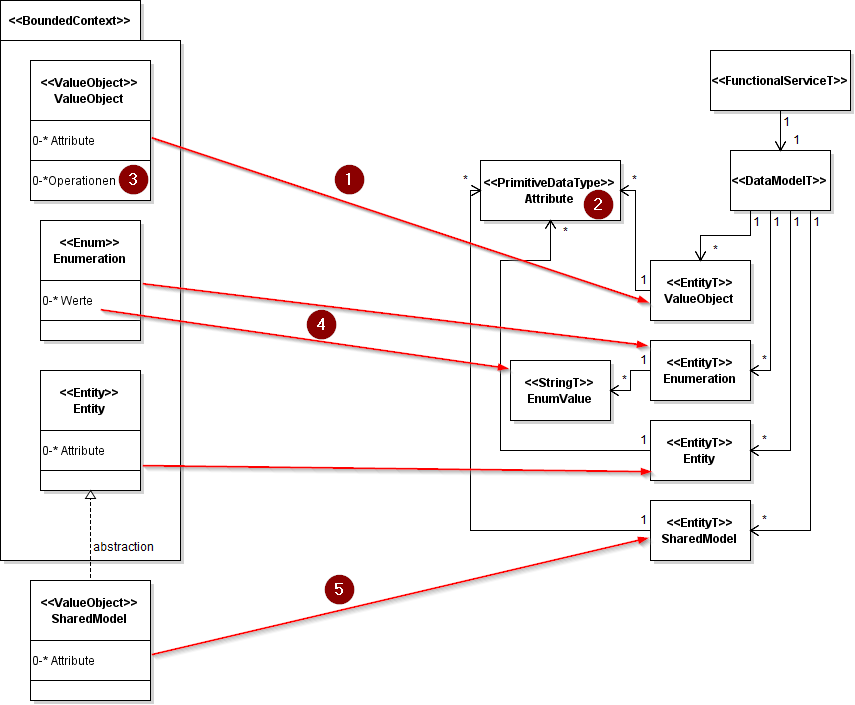
\includegraphics[width=\textwidth]{Bilder/entities_etc.png}
\caption{Transformation von ValueObjects, Specs, Enumerations und Entities}
\end{figure}
\section{Service und Repository Objekte als Schnittstellen}
\texttt{Repository} und \texttt{Service} Objekte verwalten und manipulieren in \ac{ddd} Entitäten innerhalb eines Bounded Contexts. In der Regel sind Zugriffe auf Entitäten aus anderen \texttt{Bounded Contexts} heraus nur über Objekte dieser Art möglich. \cite{DDDEvans} Wenn ein \texttt{Bounded Context} einen Microservice darstellt, können dementsprechend \texttt{Repositories} und \texttt{Services} als ServiceInterfaces verwendet werden und Aufschluss über die Abhängigkeiten zwischen den verschiedenen Microservices geben. Damit ein Microservice nur notwendige Funktionen als Interfaces bereitstellt und keine geheimen Operationen freigegeben werden, sollen in der Transformation lediglich \texttt{Repository} und \texttt{Service} Objekte, die durch \ac{uml} \texttt{Dependencies} aus anderen \texttt{Bounded Contexts} referenziert werden, mit ihren Operationen in ein Interface umgewandelt werden \cite{Rademacher2017}. Der Abbildung 4.2 sind die verschiedenen Aspekte der Transformation von \texttt{Repositories} und \texttt{Services} zu entnehmen. 

\textbf{1.) und 3.)} Für Elemente vom \ac{uml} Typ \texttt{Class} mit den Stereotypen \texttt{Service} oder \texttt{Repository} die als \texttt{supplier} einer \texttt{Dependency} fungieren, werden in \ac{ajil} \texttt{ServiceInterfaceT} Elemente mit dem alten Namen und \textit{Interface} als Suffix erzeugt und diese an dem \texttt{FunctionalServiceT}, der dem ursprünglichen \texttt{Bounded Context} entspricht als \texttt{providedInterfaces} hinzugefügt. Bei beiden Stereotypen werden die Operationen in Abilities umgewandelt. \textbf{2.)} Bei Operationen von \texttt{Services} der Anfang des Methodennamens untersucht (Die Schlagwörter nach denen kategorisiert wird, sind in der Tabelle 4.1 zu finden), um festzustellen um welchen Typ von \texttt{Ability} es sich in \ac{ajil} handeln wird. Es wird nur auf den Anfang des Methodennamens betrachtet, um die Fehleinordnung von Operationen, welche zum Beispiel \texttt{deleteReader} heißen vorzubeugen. Bei den mit \textbf{2} und \textbf{4} markierten Transformationen ist ein weiterer Entscheidungspunkt zu erkennen. Bei Operationen, bei denen nicht durch \texttt{type} ein Rückgabetyp modelliert ist (\textbf{2}), wird als \texttt{subject} der \texttt{Ability} das transformierte Ziel der ersten \texttt{Association} des \texttt{Services} oder \texttt{Repositories} verwendet. Andernfalls wird das transformierte Rückgabe Objekt zum \texttt{subject}. \textbf{5.)} Der Microservice aus dem \texttt{Bounded Context}, der in \ac{uml} die Abhängigkeiten zu den Objekten besitzt, speichert diese als \texttt{serviceDependencies}. Da abgesehen von Interfaces in \ac{ajil} kein Konzept existiert, welches \texttt{Services} oder \texttt{Repositories} innerhalb eines \texttt{DataModels} entspricht, entfällt die Transformation von Elementen, zu denen keine Abhängigkeiten aus anderen \texttt{Bounded Contexts} besteht, und es wird lediglich ein Vermerk auf die verlorenen Informationen in der Logging-Datei der Transformation erzeugt.

\begin{table}
\centering
\begin{tabular}{*5l}   \toprule
\emph{Ability} & \emph{Schlagwörter} \\\midrule
 CreateT    & \textit{create}  \\ 
 ReadT    & \textit{find}, \textit{read}, \textit{get} \\
 UpdateT    & \textit{update} \\ 
 DeleteT    & \textit{delete}, \textit{remove} \\ 
 CustomT & keine \\\bottomrule
 \hline
\end{tabular}
\caption{Schlagwörter zur Bestimmung des Ability Typen}
\end{table}
\begin{figure}
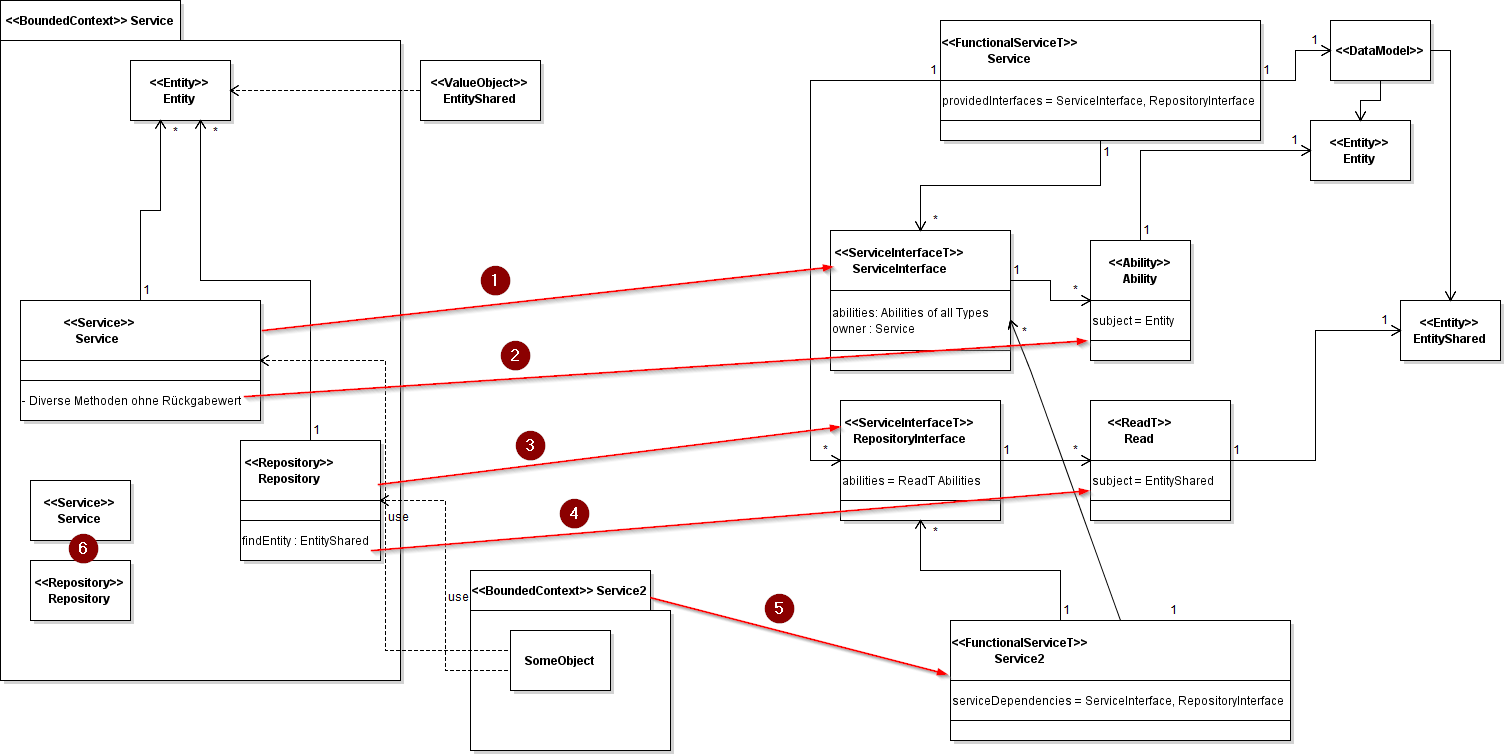
\includegraphics[width=\textwidth]{Bilder/servicesAndRepos.png}
\caption{Transformation von Repositories und Services}
\end{figure}
\section{Umgang mit Aggregaten}
Wenn ein \texttt{Bounded Context}, der Aggregate beinhaltet in einen \texttt{FunctionalServiceT} transformiert wird,  werden in seinem \texttt{DataModelT} bereits \texttt{EntityT} Elemente, welche die abstrakten Klassen AbstractAggregateRoot und AbstractAggregatePart repräsentieren sollen (\textbf{3 und 4}). Hierbei ist zu vermerken, dass \ac{ajil} keine abstrakten Klassen unterstützt, jedoch abstrakte Klassen in der späteren Implementierung der \ac{msa} nützlich sind, um von Evans formulierte Fähigkeiten von Aggregaten, wie zum Beispiel alle \texttt{AggregateParts} einer \texttt{AggregateRoot}erhalten zu können, allgemeingültig zu realisieren. \textbf{1.) und 2.)} \texttt{Entities}, die zusätzlich die Stereotypen \texttt{AggregateRoot} oder \texttt{AggregatePart} besitzen, werden in \texttt{EntityT} Elemente transformiert und um sie als  \texttt{AggregateRoot} oder \texttt{AggregatePart} zu kennzeichnen, wird der Wert für \texttt{parent} auf die jeweilige abstrakte Klasse gesetzt, wodurch eine \texttt{extends} Beziehung entsteht.
\begin{figure}
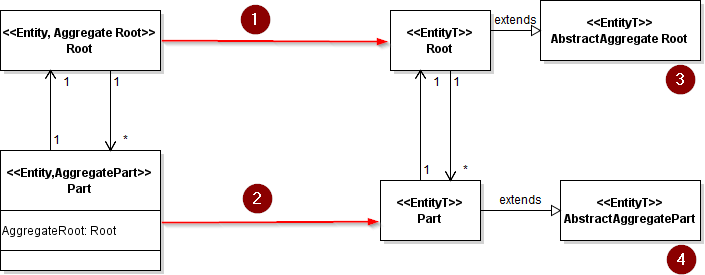
\includegraphics[width=\textwidth]{Bilder/aggregates_rules_explained.png}
\caption{Transformation von Aggregaten}
\end{figure}
\section{Sonstige Transformationen}
In der Baumstruktur einer \textit{.ajimlt} Datei stellt das \texttt{SystemT} Element die Wurzel dar. Da in \ac{uml} dies dem Typen \texttt{Model} entspricht, wird ein \texttt{Model} in ein \texttt{SystemT} transformiert. Zudem werden die \texttt{Abstractions} von implementierenden \texttt{Entities} zu abstrakten \texttt{Entities} durch das Setzen des \texttt{parent} Attributs an der \texttt{Entity} in \ac{ajil} auf das Elternelement ausgedrückt. Da in \ac{ajil} keine entsprechenden Konzepte für die Stereotypen \texttt{Closure}, \texttt{SideEffectFree},\texttt{definesIdentity} oder \texttt{validatesSpec} existieren, werden diese Stereotypen nicht nach gesonderten Regeln transformiert, sondern nach ihrem \ac{uml}-Typ ausgewertet.
\section{Tabellarischer Überblick über Regeln}
Der Tabelle 4.2 sind die umzusetzenden Transformationsregeln anhand von \ac{uml}-Typ und angewandtem \ac{uml}-Stereotyp des Quellelements zum \ac{ajil} Zielelements mit Anmerkungen zu entnehmen.
\begin{table}
\begin{tabular}{*5l}   \toprule
\emph{\ac{uml}-Typ} & \emph{\ac{uml}-Stereotyp} & \emph{\ac{ajil}-Elemente}  \\\midrule
 Model    & - & SystemT  \\ 
 Package & Bounded Context & FunctionalServiceT + DataModelT \\
 Package & Module & - \\
 Class & Entity & EntityT \\
 Class & Entity, AggregateRoot & EntityT (parent = AbstractAggregateRoot) \\
 Class & Entity, AggregatePart & EntityT (parent = AbstractAggregatePart) \\
 Class & Value Object & EntityT \\
 Class & Spec & - \\
 Class & Repository oder Service & ServiceInterfaceT (wenn Dependencies existieren) \\
 Property & \textit{irrelevant} & PrimitiveDataType (Default StringT) \\
 Operation & \textit{irrelevant} & Ability (nur Repositories, Services; Default CustomT) \\
 Abstraction & - & supplier als parent an EntityT \\
 Association & - & Association (Nur Entities, Enumerations, ValueObjects) \\
 Dependency & - & ServiceDependency (wenn zwischen Bounded Contexts) \\\bottomrule
 \hline
\end{tabular}
\caption{Transformationen Im Überblick}
\end{table}


\chapter{Implementierung des Konzepts}
\section{Auswahl eines geeigneten Transformationstools}
\subsection{Kriterien}
In \cite{MDEToolEvaluation} werden verschiedene \ac{mdsd} Tools zusammengetragen und kategorisiert. Hierbei werden verschiedene Kriterien zur Auswahl von \ac{mdsd} Tools formuliert. Im Folgenden werden die Kriterien vorgestellt und beschrieben, inwieweit diese für das \ac{mdsd} Tool, welches in dieser Arbeit zum Einsatz kommen soll, erfüllt werden sollen.
\paragraph{M2M oder M2T?} 
So wie Transformationen an sich, lassen sich Transformationssprachen darin unterscheiden ob sie ein Model in ein anderes Model umwandeln, oder in Text. Da von einem \ac{uml} Modell in ein \ac{ajil} Modell transformiert werden soll, muss die Sprache für \ac{m2m} Transformationen geeignet sein.
\paragraph{Transformationsansatz} 
Im Bereich der \ac{m2m} Transformationen wird hinsichtlich der für Transformationen verwendeten Sprachkonstrukte und Mechanismen zwischen relational, imperativ, graphbasiert oder hybriden Ansätzen unterschieden. Da der Autor dieser Arbeit hauptsächlich Erfahrung mit imperativen Ansätzen hat, sollte die gewählte Sprache imperativ oder hybrid mit der Möglichkeit komplexe Transformationsoperationen imperativ zu beschreiben sein.
\paragraph{Generelle Bedingungen} 
In dieser Kategorie befinden sich Kriterien, die mit nicht technischen Aspekten der verwendeten Technologie zusammenhängen, wie Lizensierung und Support. Da die beiden Ansätze, die transformiert werden sollen noch in der Entwicklung befinden und eine Anforderung an die Transformation eine zukunftssichere Erweiterbarkeit darstellt, sollte die Technologie weiterhin vom Hersteller unterstützt werden. Zusätzlich kann bei Schwierigkeiten bezüglich der Entwicklung auf vom Hersteller zur Verfügung gestellte Dokumentation und Unterstützung zurückgegriffen werden. Zudem sollte es sich bei der Technologie um ein Open Source Produkt ohne Lizensierungskosten handeln, da keine monetären Ressourcen bestehen und um die Portabilität der Transformation einfacher zu gestalten.
\paragraph{Modellierungsaspekte}
Diese Kategorie umfasst sämtliche Eigenschaften bezüglich der Unterstützung verschiedener Aspekte der Modellierung, wie Kompatibilität mit bestimmten Modellierungssprachen, Metametamodellen oder bestehenden Standards zum Informationsaustausch auf Modellebene. Das verwendete Tool muss \ac{uml} (\ac{mof})und Ecore unterstützen, um die den zu transformierenden Modellen zugrunde liegenden Metamodelle auswerten und anwenden zu können. Hieraus ergibt sich, dass das \ac{mof} Metametamodell unterstützt werden sollte.
\paragraph{Transformationsaspekte}
Diese Facette umfasst alle Anforderungen an die durchgeführten Transformationen, bezüglich der Art der Syntax, Kardinalität etc.. Bezüglich der Syntax ist eine textuelle Darstellung ausreichend, da die implementierte Transformation nur von Entwicklern erweitert werden soll. Da ein Modell in ein anderes überführt wird, ist eine Kardinalität von eins zu eins notwendig und nicht die Erzeugung oder Eingabe von mehreren verschiedenen Modellen. Der Output des Modells kann konservativ erfolgen, das heißt, dass ein neues Modell erzeugt wird und kein bestehendes verändert, da eine neue Datei unter einem anderen Metamodell erstellt werden muss. Regelapplikationskontrolle muss unterstützt werden, da gleiche Elemente unter verschiedenen Bedingungen unterschiedlich transformiert werden, wie zum Beispiel beim unterschiedlichen Umgang mit \texttt{ValueObjects} und Shared Models. Das Tool muss exogene Transformationen unterstützen, da beiden Modellen verschiedene Metamodelle zugrunde liegen. Die Fähigkeit zur Durchführung von Unidirektionalen Transformationen genügt.
\paragraph{User Experience Aspekte}
An dieser Stelle wird Nutzerfreundlichkeit des Tools betrachtet, diese Aspekte stellen für die Evaluation an dieser Stelle eine untergeordnete Rolle. Für eine effektive Entwicklung sollten jedoch bestimmte Faktoren gegeben sein: Das Tool sollte über einen Syntax und Semantik sensitiven Editor mit Error Warnungen, Syntax Higlighting, Autovervollständigung etc. verfügen. Darüber hinaus sollte durch komplexere Transformationsbedingungen und den Hintegrund des Autors dieser Arbeit der Programmierstil Programmiersprachenähnlich sein.
\paragraph{Kollaborationsaspekte}
Diese Facette beschreibt wie gut sich das Tool in Projekte einbinden und für diese erweitern lässt. 
Um Transformation und Entwicklungsfortschritte zu sichern, sollten die vom Tools verwendeten Dateien kompatibel mit Versionskontrolltools sein.
\paragraph{Laufzeitsaspekte}
Zuletzt wird betrachtet unter welchen Umständen das Tool ausgeführt werden soll.
Enweder soll die implementierte Transformation als standalone Applikation ohne viel Konfigurationsaufwand oder über Eclipse, da sowohl \ac{uml} Modelle, als auch \ac{ajil} in Eclipse Umgebung integriert sind, ausführbar sein. Zudem sollte sowohl die Entwicklung, als auch die Ausführung der Transformation betriebssystemunabhängig möglich sein. 

%\subsection{Optionen}
%\cite{MDEToolEvaluation} stellt auch Website zur Verfügung, die Filter anwenden kann, diese wurde verwendet, um eine Vorauswahl an Tools zu treffen. Viele Tools entfallen, weil sie durch einen Fokus auf \ac{dsml}s lediglich Ecore verwenden.
%ATL
%Kermeta
%QVTO

%Raus, weil discontinued:
%- Age (agile generative environment) seit 2009
\subsection{Entscheidung}
\cite{MDEToolEvaluation} stellt zusätzlich zu der Veröffentlichung eine Website\footnote{www.mdetools.com} zur Verfügung, auf der der Klassifizierung der Tools entsprechendete Filter verwendet werden können. Diese wurde verwendet, um eine Vorauswahl an Tools zu treffen. Viele Tools entfallen, weil sie durch einen Fokus auf \ac{dsml}s lediglich Ecore verwenden. Ebenfalls sind viele Tools im Bereich \ac{mdsd} zum Zeitpunkt der Erstellung dieser Thesis nicht mehr unterstützt.

Für die Implementierung der Transformation soll die \ac{atl} verwendet werden. Es handelt sich um eine Transformationssprache, welche auf \ac{m2m} Transformationen ausgelegt ist und eine Komponente der \ac{m2m} Implementierung des \ac{omg} \ac{qvt} Standards im \ac{emp} darstellt, womit sie unter die kostenfreie Eclipse Lizenz fällt. Dadurch ist die Transformation mit der Eclipse \ac{ide} in der selben Umgebung programmier- und ausführbar wie die beiden zu transformierenden Tools. Mit der Arbeit in der Eclipse \ac{ide} gehen alle Eigenschaften und Vorteile bezüglich der Laufzeit und Benutzerfreundlichkeit des Editors, die Eclipse bietet mit der Verwendung von \ac{atl} einher. Darüber hinaus kann durch die Verwendung der vom  \ac{emf} zur Verfügung gestellten \ac{emftvm} theoretisch eine \ac{ide} unabhängige Ausführung implementiert werden. \ac{atl} verfügt über die Möglichkeit exogene \ac{m2m} Transformationen durchzuführen, wobei nicht nur Metamodelle des \ac{emf} wie Ecore verwendet werden können, deonrn auch \ac{uml}. Der Transformationsansatz ist hierbei hybrid, wobei Elemente grundsätzlich nach deklarativ beschriebenen Regeln transformiert werden, jedoch auch imperativer Code verwendet werden kann, um komplexe Transformationsbedingungen zu erfüllen. \cite{ATLDoc}

Für den imperativen Code wird ähnlich dem \ac{uml}-Profils für \ac{ddd} und der Validierung in \ac{ajil} Ausdrücke der Sprache \ac{ocl} verwendet, wodurch Entwickler mit Expertise in diesem Bereich eine Grundlage für die Arbeit mit \ac{atl} besitzen. Um die Einarbeitung in die Sprache zu erleichtern, existieren zu \ac{atl} zahlreiche Fallbeispiele \footnote{www.eclipse.org/atl/atlTransformations} und ein reges Subforum im Eclipse Forum \footnote{www.eclipse.org/forums/index.php/f/241}.


\section{Atlas Transformation Language}
\subsection{Funktionsweise}


Konfiguration und Funktionsweise der Transformation ist demnachin der Abbildung 5.1 gemäß \cite{transformationModels} zu erkennen. Hier folgt noch eine ausführlichere Beschreibung.
\begin{lstlisting}[caption={Kopf des ATL Moduls},captionpos=b,label=Quellcode:ModuleKopf] 
module ddd2ajimlt;
create OUT : AJI from IN : DDD;
\end{lstlisting}
\begin{figure}
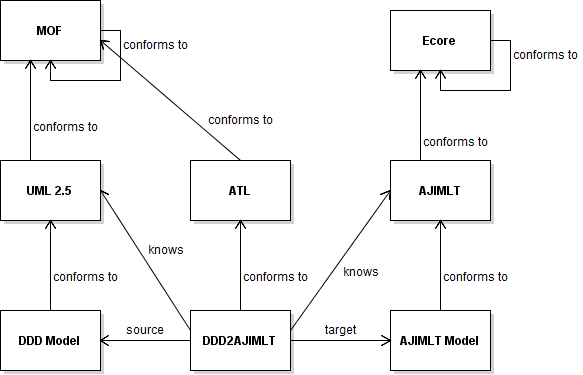
\includegraphics[width=\textwidth]{Bilder/transformationModelOverview.png}
\caption{Transformationsmodellübersicht}
\end{figure}
\subsection{Aufbau von Regeln}
In der Implementierung werden die von \ac{atl} verwendeten \textbf{Matched Rules} verwendet. Sie erzeugen für bestimmte Eingabe Elemente eine bestimmte Menge an Ausgabe Elementen. 

Die Auswahl der durch eine Regel zu transformierenden Elemente geschieht über das \textbf{Source Pattern} jeder Regel. Dieser Teil wird durch ein \texttt{from} deklariert und spezifiziert zunächst einen Elementtyp im Eingabemodell und den Variablennamen für das Element, welcher in der Regel verwendet wird um das Element zu referenzieren. Für jedes Element dieses Typen werden anschließend mithilfe von Aussagenlogik verschiedene Kriterien geprüft, die das Element erfüllen muss. Zu beachten ist hier, dass bei Ausdrücken in \ac{atl} generell der komplette Ausdruck in der Klammer ausgewertet wird, wodurch die Gefahr von Exceptions (z.B. Null-Pointern) bei der Auswertung der Eigenschaften eines Elements bedacht werden muss. 

Wenn das Element im Eingabemodell die Bedingungen der Regel erfüllt, wird der \textbf{Target Pattern} Teil der Regel ausgeführt (durch die Verwendung von \texttt{to} eingeleitet), in welchem die Elemente des Ausgabemodells, welche durch die Regel erzeugt werden beschrieben werden. Hierbei wird zunächst ähnlich der Syntax im Source Pattern ein Variablenname und ein Elementtyp festgelegt. In den darauf folgenden Klammern können die Eigenschaften des zu erzeugenden Elements gesetzt werden, wobei auch auf Eigenschaften des Eingabeelements ausgewertet werden können. Darüber hinaus kann eine Regel über einen Teil zur Deklaration von weiteren im Target Pattern verwendeten Variablen verfügen, dieser wird über \texttt{using} eingeleitet, und imperativ implementiert.
\cite{ATLDoc}
\subsection{Aufbau von Helpern}
\ac{atl} bietet Entwicklern durch die Definition sogenannter \textbf{Helper} imperativen Code zu schreiben, der durch die Funktionalität bestimmter Datentypen erweitern kann. Somit sind Helper an jeder Stelle im \ac{atl} Modul anwendbar und können bei der Validierung im Source oder der Beschaffung der gewünschten Werte im Target Pattern verwendet werden, obwohl innerhalb dieser selbst kein imperativer Code verwendet wird. Durch \texttt{Context context\_type} kann angegeben werden, von welchem Datentyp der Helper angewendet werden kann. Das aufrufende Objekt selbst kann anschließend über \texttt{self} ausgewertet werden. Wird dieser Wert nicht angegeben, ist der Helper dem globalen Kontext des \ac{atl} Moduls zugeordnet, und wird durch das Objekt \texttt{thisModule}, welches an jedem Punkt des Moduls verfügbar ist, aufgerufen. Darüber hinaus können neben dem Namen beliebig viele durch Komma separierte Parameter angegeben werden und ein Return Type angegeben werden. Der Körper \texttt{exp} eines Helpers besteht aus einem \ac{ocl} Ausdruck, welcher den Rückgabewert des Helpers liefert. \cite{ATLDoc}
\begin{lstlisting}[caption={Schema zur Deklaration von Helpern \cite{ATLDoc} },captionpos=b,label=Quellcode:HelperSchema] 
helper[context context_type]? def :helper_name(parameters) :return_type =exp;\end{lstlisting}
\section{Implementierung der Regeln}
\subsection{Traversierung des Eingabemodells}
Da bei der Konzeptionierung der Transformation zwischen den Modellen komplexe Zusammenhänge und Informationen betrachtet werden, welche an in der Baumstruktur des \ac{uml} Modells teils nicht beieinander liegenden Stellen gepflegt sind (vgl. Abschnitt X.X) ist es notwendig das \ac{uml} Modell effektiv traversieren zu können. In den Elementen eines \ac{ddd}-{uml} Modells, die es zu transformieren gilt, kann die Eigenschaft \texttt{namespace} verwendet werden, um Informationen über das Elternelement eines Elements zu erhalten. Da jedoch ein wiederholtes manuelles Aufrufen des \texttt{namespace} eines Elements, z.B. von einer \texttt{Entity} bis zu dem enthaltenden \texttt{Bounded Context} weder leserlichen Code, noch eine dynamische und fehlerresistente Methode der Traversierung darstellt, werden im \ac{atl} Modul zwei verschiedene rekursive Helper verwendet, um ein \ac{uml} Modell "nach oben" zum Kern hin zu traversieren:
 \texttt{goUpToElementWithStereotype} für angewendete Stereotypen und \texttt{goUpToElementWithType} für \ac{uml} Typen. 
 
 Die Methoden überprüfen ob das aufrufende Element selbst den gesuchten Stereotyp/\ac{uml}-Typ hat. \texttt{GoUpToElementWithStereotype} verwendet an dieser Stelle einen selbst implementierten Helper \texttt{hasStereotype}. Falls das Element den Typ hat, wird es zurückgeliefert, ansonsten, falls der \texttt{namespace} des Elements nicht leer (\texttt{oclUndefined}) ist, soll der selbe Helper für das Elternelement aufgerufen werden. Damit dies möglich ist, sind die Helper für jeden Elementtyp in \ac{uml} als Context definiert. Falls der \texttt{namespace} des Elements leer ist, bedeutet dies, dass ohne Ergebnis bis zum Kern des \ac{uml} Modells navigiert wurde In diesem Fall soll OclUndefined zurückgeliefert werden.
\begin{lstlisting}[caption={Helper zur rekursiven Suche nach Elternelementen},captionpos=b,label=Quellcode:GoUpToElementWithStereotype] 
helper context UML!Element def: goUpToElementWithStereotype (stereotype : String) : DDD!Element =
	if(self.hasStereotype(stereotype))
		then
			self
		else
			if(not self.namespace.oclIsUndefined())
				then
					self.namespace.goUpToElementWithStereotype(stereotype)
				else
					OclUndefined
				endif
		endif;
\end{lstlisting}
Zusätzlich sind besondere Helper für das effektive Sammeln von Elementen in \texttt{Bounded Contexts} notwendig, denn obwohl über die Eigenschaft \texttt{packagedElement} von \texttt{Packages} sämtliche vom \texttt{Package} beinhalteten Elemente ausgewertet werden können, kann es sein, dass innerhalb eines \texttt{Bounded Context} Elemente durch verschiedene \texttt{Modules} organisiert sind. Aus diesem Grund werden im Modul für das Sammeln von Elementen mit bestimmten Stereotypen oder \ac{uml}-Typen durch mehrere \texttt{Packages} rekursive Helper zur Verfügung gestellt. Hierbei wird über \texttt{packagedElement} des aufrufenden Elements iteriert, und falls das beinhaltete Element den gesuchten Typ besitzt wird es einer \texttt{Collection} hinzugefügt. Falls es sich um ein weiteres \texttt{Package} handelt wird von dem Element aus der Helper erneut aufgerufen und die Ergebnis \texttt{Collection} dieses Aufrufs mit der bestehenden vereint.
\begin{lstlisting}[caption={Helper zur rekursiven Suche nach Kindelementen},captionpos=b,label=Quellcode:getPackagedELementsByType] 
helper context DDD!Element def: getPackagedElementsByType(type : String) : Sequence(DDD!Class) =
		self.packagedElement ->
			iterate(iter; col: Sequence(DDD!Element) = Sequence{}|
		if(iter.oclIsTypeOf(type))
			then
				col.append(iter)
		else
			if(iter.oclIsTypeOf(DDD!Package))
				then
				col.union(iter.getPackagedElementsByType(type))
			else
				col
			endif
		endif);
\end{lstlisting}
\subsection{Nutzung von Traceability Links}
Bei der Transformation eines Elements erstellt \ac{atl} Traceability Links, um das Element aus dem Eingabemodell mit den im Target Pattern erzeugten Elementen des Ausgabemodells zu verknüpfen. Diese Links können verwendet werden, um Verbindungen zwischen Elementen im Eingabemodell bei der Transformation beizubehalten. Der Helper \texttt{getPackagedElementsByStereoType} liefert sämtliche \ac{uml} Elemente, die das Eingabeelements. Wenn zum Beispiel bei dem aus einem \texttt{BoundedContext} Element in \ac{ajil} erzeugten \texttt{DataModelT} die Eigenschaft \texttt{entities} mit dem Ergebnis des Helpers befüllt wird (vgl. Quellcode 5.4, Zeile 16), kann \ac{atl} für jede \ac{uml} \texttt{Entity} bestimmen, welches Element durch eine Regel (z.B Quellcode 5.5), die die \texttt{Entity} im Source Pattern akzeptiert hat erzeugt wurde und diese einsetzen.  
\begin{lstlisting}[caption={Regel zur Erzeugung eines Microservices},captionpos=b,label=Quellcode:BoundedContext2MicroServiceAndDataModelWithoutAggregate] 
rule BoundedContext2MicroServiceAndDataModelWithoutAggregate {
	from
		p : DDD!Package (p.oclIsTypeOf(DDD!Package) and p.hasStereotype('BoundedContext') and p.getPackagedElementsByStereoType('AggregateRoot').size() = 0)
	to
		
		fs: AJI!FunctionalServiceT (
			name <- p.name + 'Service',
			domain <- dm,
			providedInterfaces <- p.getPackagedElementsByStereoType('Repository'),
			providedInterfaces <- p.getPackagedElementsByStereoType('Service'),
			serviceDependencies <- p.getDependenciesToOtherContexts()
		),
		
		dm:	AJI!DataModelT (
			name <- p.name + 'Model',
			entities <- p.getPackagedElementsByStereoType('Entity'),
			entities <- p.getPackagedElementsByStereoType('ValueObject'),
			entities <- p.getPackagedElementsByType(DDD!Enumeration)
		)
}
\end{lstlisting}
Wenn aus einem Eingabeelement durch eine Regel mehrere Ausgabeelemente erzeugt wurden, kann der Helper \texttt{resolveTemp} genutzt werden, um anhand des Variablennamens zu bestimmen, welcher Traceability Link verwendet werden soll (vgl. Quellcode 5.5, Zeile 11). Würde ein Element von mehreren Regeln akzeptiert werden und dadurch verschiedene Links entstehen, kann ebenfalls \texttt{resolveTemp} verwendet werden, mit dem Namen der Regel als Parameter. Während \texttt{Entity}, \texttt{ValueObject} und \texttt{Enumeration} Elemente durch Traceability Links dem entsprechenden \texttt{DataModelT} hinzugefügt werden, wird bei Klassen, die abstrakte Klassen spezifizieren das DataModel schon bei der Erzeugung der \texttt{EntityT} auf das DataModel der generalisierenden Klasse gesetzt. Dies wird an dieser Stelle implementiert, da der Filterungsaufwand vom \texttt{BoundedContext} aus größer wäre.
\begin{lstlisting}[caption={Regel zur Erzeugung einer einfachen Entity},captionpos=b,label=Quellcode:Entity2Entity_NoAggregate] 
rule Entity2Entity_NoAggregate{
	from
		old : DDD!Class ((old.hasStereotype('Entity') or old.generalizationHasStereotype('Entity')) 
			and not (old.hasStereotype('AggregateRoot') or old.hasStereotype('AggregatePart')))
	to
		new : AJI!EntityT(
				name <- old.name,
				attributes <- old.attribute,
				relations <- old.getAllAssocationsFromProperties(),
				parent <- old.getGeneralization(),
				domainModel <- thisModule.resolveTemp(old.generalizationBoundedContext(), 'dm')
			)
}
\end{lstlisting}
\subsection{Transformation von Shared Models}
Die Unterscheidung von normalen \texttt{ValueObjects} und Shared Models ist notwendig, da Shared Models speziellen Transformationregeln unterliegen (vgl. Abschnitt 4.2, Punkt 6). Ein Shared Model zeichnet sich nicht durch einen gesonderten Stereotypen aus, spondern dadurch, dass es als \texttt{ValueObject} zwischen \texttt{Bounded Contexts} besteht \cite{DDDEvans}. Diese Eigenschaft wird genutzt, um aus \texttt{ValueObject} Elementen Shared Models zu identifizieren, da der Helper \texttt{goUpToElementWithStereotype}, wenn kein Elternelement mit dem Stereotyp \texttt{BoundedContext} gefunden wird, \texttt{OclUndefined} zurückgibt (vgl. Quellcode 5.6, Zeile 3). 

Als für die Regel gültige Variable wird mit \texttt{abstraction} der \texttt{supplier} eines \texttt{Abstraction} Elements gesetzt, welches das Shared Model als \texttt{client} definiert (vgl. Zeile 5) Hierzu wird im zur Initialisierung der Variable verwendeten Helper bis zum Element mit dem \ac{uml}-Typen \texttt{Model} gegangen, und von hier aus der rekursive Helper \texttt{getPackagedElementsByType} aufgerufen um alle \texttt{Abstractions} des Modells zu erhalten. Die entstandene \texttt{Collection} wird zuletzt hinsichtlich des \texttt{client} gefiltert. Es gilt zu beachten, dass es im Falle von mehreren Treffern keine Möglichkeit gibt zu bestimmen, welche \texttt{Abstraction} im weiteren Verlauf der Regel verwendet werden soll, weswegen in diesem Fall nur das erste Element zurückgegeben wird.

Bei der Erzeugung des Ausgabeelements wird anschließend \texttt{parent} auf die Klasse von der das SharedModel abgeleitet ist und \texttt{domainModel} auf das \texttt{domainModel} gesetzt, welches aus dem \texttt{BoundedContext} Element, dem sie zugeordnet ist,erzeugt wird. Da \ac{atl} bei der Transformation zunächst Platzhalter Elemente für jede ausgeführte Regel anlegt, und in einem weiteren Schritt die Eigenschaften dieser setzt \cite{ATLDoc}, musste das \texttt{domainModel} einer \texttt{Entity} in \ac{ajil} auf \texttt{changeable = true} geändert werden, da ansonsten eine Änderung des \texttt{domainModel} nach der Initialisierung nicht möglich wäre.
\begin{lstlisting}[caption={Regel zur Erzeugung einer Entity aus einem Shared Model},captionpos=b,label=Quellcode:SharedModel2Entity] 
rule SharedModel2Entity{
	from
		old : DDD!Class (old.hasStereotype('ValueObject') and old.goUpToElementWithStereotype('BoundedContext').oclIsUndefined())
	using{
		abstraction : DDD!Abstraction = thisModule.getAbstractFromSharedModel(old).supplier.get(0);
	}	
	to
		new : AJI!EntityT(
				name <- old.name,
				attributes <- old.attribute,
				domainModel <- thisModule.resolveTemp(abstraction.goUpToElementWithStereotype('BoundedContext'), 'dm'),
				parent <- abstraction
			)
}
\end{lstlisting}
\subsection{Erzeugung von Interfaces und Abilities}
Bei der Erzeugung von \texttt{ServiceInterfaces} aus \texttt{Repository} oder \texttt{Service} Klassen wird über den Helper \texttt{suitableForInterface} gefiltert (vgl. Quellcode 5.7, Zeile 3). Dieser prüft zunächst, ob das Element einen der beiden Stereotypen besitzt und ruft in diesem Fall durch das Element den Helper \texttt{countDependenciesOnThis} (Quelllcode 5.8) auf . Dieser sammelt zunächst vom kompletten \texttt{Model}, in welchem sich das Element befindet, \texttt{Dependencies}. Die \texttt{Dependencies} werden anschließend danach gefiltert, ob das aufrufende Element als \texttt{supplier} gesetzt ist, wodurch es eine \texttt{Dependency} auf das aufrufende Element ist, und ob \texttt{supplier} und \texttt{client} verschiedenen \texttt{Bounded Contexts} zugeordnet sind, wodurch es sich um eine Service Dependency handelt. Wenn die dadurch entstandene \texttt{Collection} nicht leer ist, wird aus dem Element ein \texttt{ServiceInterfaceT} erzeugt, andernfalls wird eine LOG Ausgabe erzeugt, die über den Informationsverlust des Elements informiert. Die \texttt{abilities} des \texttt{ServiceInterfaceT} werden durch Traceability Links zu den \texttt{Operations}, die das \ac{uml} Element besitzt, zugeordnet.
\begin{lstlisting}[caption={Regel zur Erzeugung eines Service Interface},captionpos=b,label=Quellcode:RepositoryOrService2ServiceInterface] 
rule RepositoryOrService2ServiceInterface{
	from
		old : DDD!Class (old.suitableForInterface())
	to
		new : AJI!ServiceInterfaceT(
				name <- old.name + 'Interface',
				abilities <- old.ownedOperation
			)
}
\end{lstlisting}
\begin{lstlisting}[caption={Helper zum Zählen von Interface Dependencies},captionpos=b,label=Quellcode:countDependenciesOnThis] 
helper context DDD!Class def: countDependenciesOnThis() : Boolean =
	self.goUpToElementWithType(DDD!Model).getPackagedElementsByType(DDD!Dependency) -> 
	iterate(iter; col: Sequence(DDD!Class) = Sequence{}|
		if(iter.supplier.get(0).name = self.name)
			then
				if(thisModule.sameBoundedContextNames(iter.supplier.get(0), iter.client.get(0)))
					then
						col.append(iter)
					else
						col
					endif
			else
				col
			endif);
\end{lstlisting}
Stellvertretend für die verschiedenen Regeln zur Transformation von \texttt{Operations} in die entsprechenden \texttt{Abilities} wird an dieser Stelle die Regel \texttt{Operation2CreateAbility} erläutert. Bei der Auswertung des die jeweilige \texttt{Operation} besitzende Element, wird direkt auf \texttt{namespace} der \texttt{Operation} zugegriffen, da in \ac{uml} keine Elemente zwischen \texttt{Operations} und \texttt{Classes} modelliert werden, die die Auswertung verfälschen könnten. Zusätzlich wird der Anfang des Namens der \texttt{Operation} gemäß Tabelle 4.1 gefiltert, um in \ac{ajil} den entsprechenden \texttt{Ability} Typen zu erzeugen. Das letzte Filterkriterium ist mit Aufruf des Helpers \texttt{countDependenciesOnThis()} das gleiche wie für die Erzeugung von \texttt{Interfaces} auf dem \texttt{namespace} des Elements, um keine \texttt{Operations} zu transformieren, deren Elternelemente nicht transformiert werden. Hier wird nicht der Helper \texttt{suitableForInterface} verwendet, da dies duplizierte LOG Ausgaben erzeugen würde.
\begin{lstlisting}[caption={Regel zur Erzeugung einer Ability},captionpos=b,label=Quellcode:Operation2CreateAbility] 
rule Operation2CreateAbility{
	from
		old: DDD!Operation ((old.namespace.hasStereotype('Repository') or old.namespace.hasStereotype('Service')) 
			and old.name.substring(1,6) = 'create' 
			and old.namespace.countDependenciesOnThis().size() > 0) 
	to
		new : AJI!CreateT( 
				name <- old.name,
				subject <- old.getCorrectSubject()
			)
}
\end{lstlisting}
\begin{lstlisting}[caption={Helper für das korrekte Subject einer Ability},captionpos=b,label=Quellcode:getCorrectSubject] 
helper context DDD!Operation def: getCorrectSubject() : DDD!Element =
	if(self.type.oclIsUndefined())
		then 
			if not self.namespace.getAllAssocationsFromProperties().first().oclIsUndefined()
				then
					self.namespace.getAllAssocationsFromProperties().first().memberEnd.first().type
				else
					self.namespace.goUpToElementWithType(DDD!Model).collectAssociationsWithMemberEnd(self.namespace).first().memberEnd.get(0).type
			endif
		else
			self.type
	endif;	
\end{lstlisting}
\section{Ausführung}
\subsection{Ausführung als Standalone Jar}
An Florian und Jonas: An dieser Stelle bin ich gescheitert es standalone auszuführen und konnte keine Hilfe aus dem Eclipse Forum bekommen, ist ein negatives Ergebnis in diesem Fall auch ein Ergebnis?
%emftvm gescheitert, Grund für Fehlermeldung finden wäre gut
\subsection{Einrichtung und Ausführung in Eclipse}
Vorbedingungen und Konfiguration beschreiben
\section{Evaluation anhand eines Domänenmodells aus der Praxis}
Hier wird beschrieben, wie evaluiert wurde, vielleicht auch noch das Testdiagramm für Aggregate rein packen + Ausführungsdauer messen.
\begin{figure}
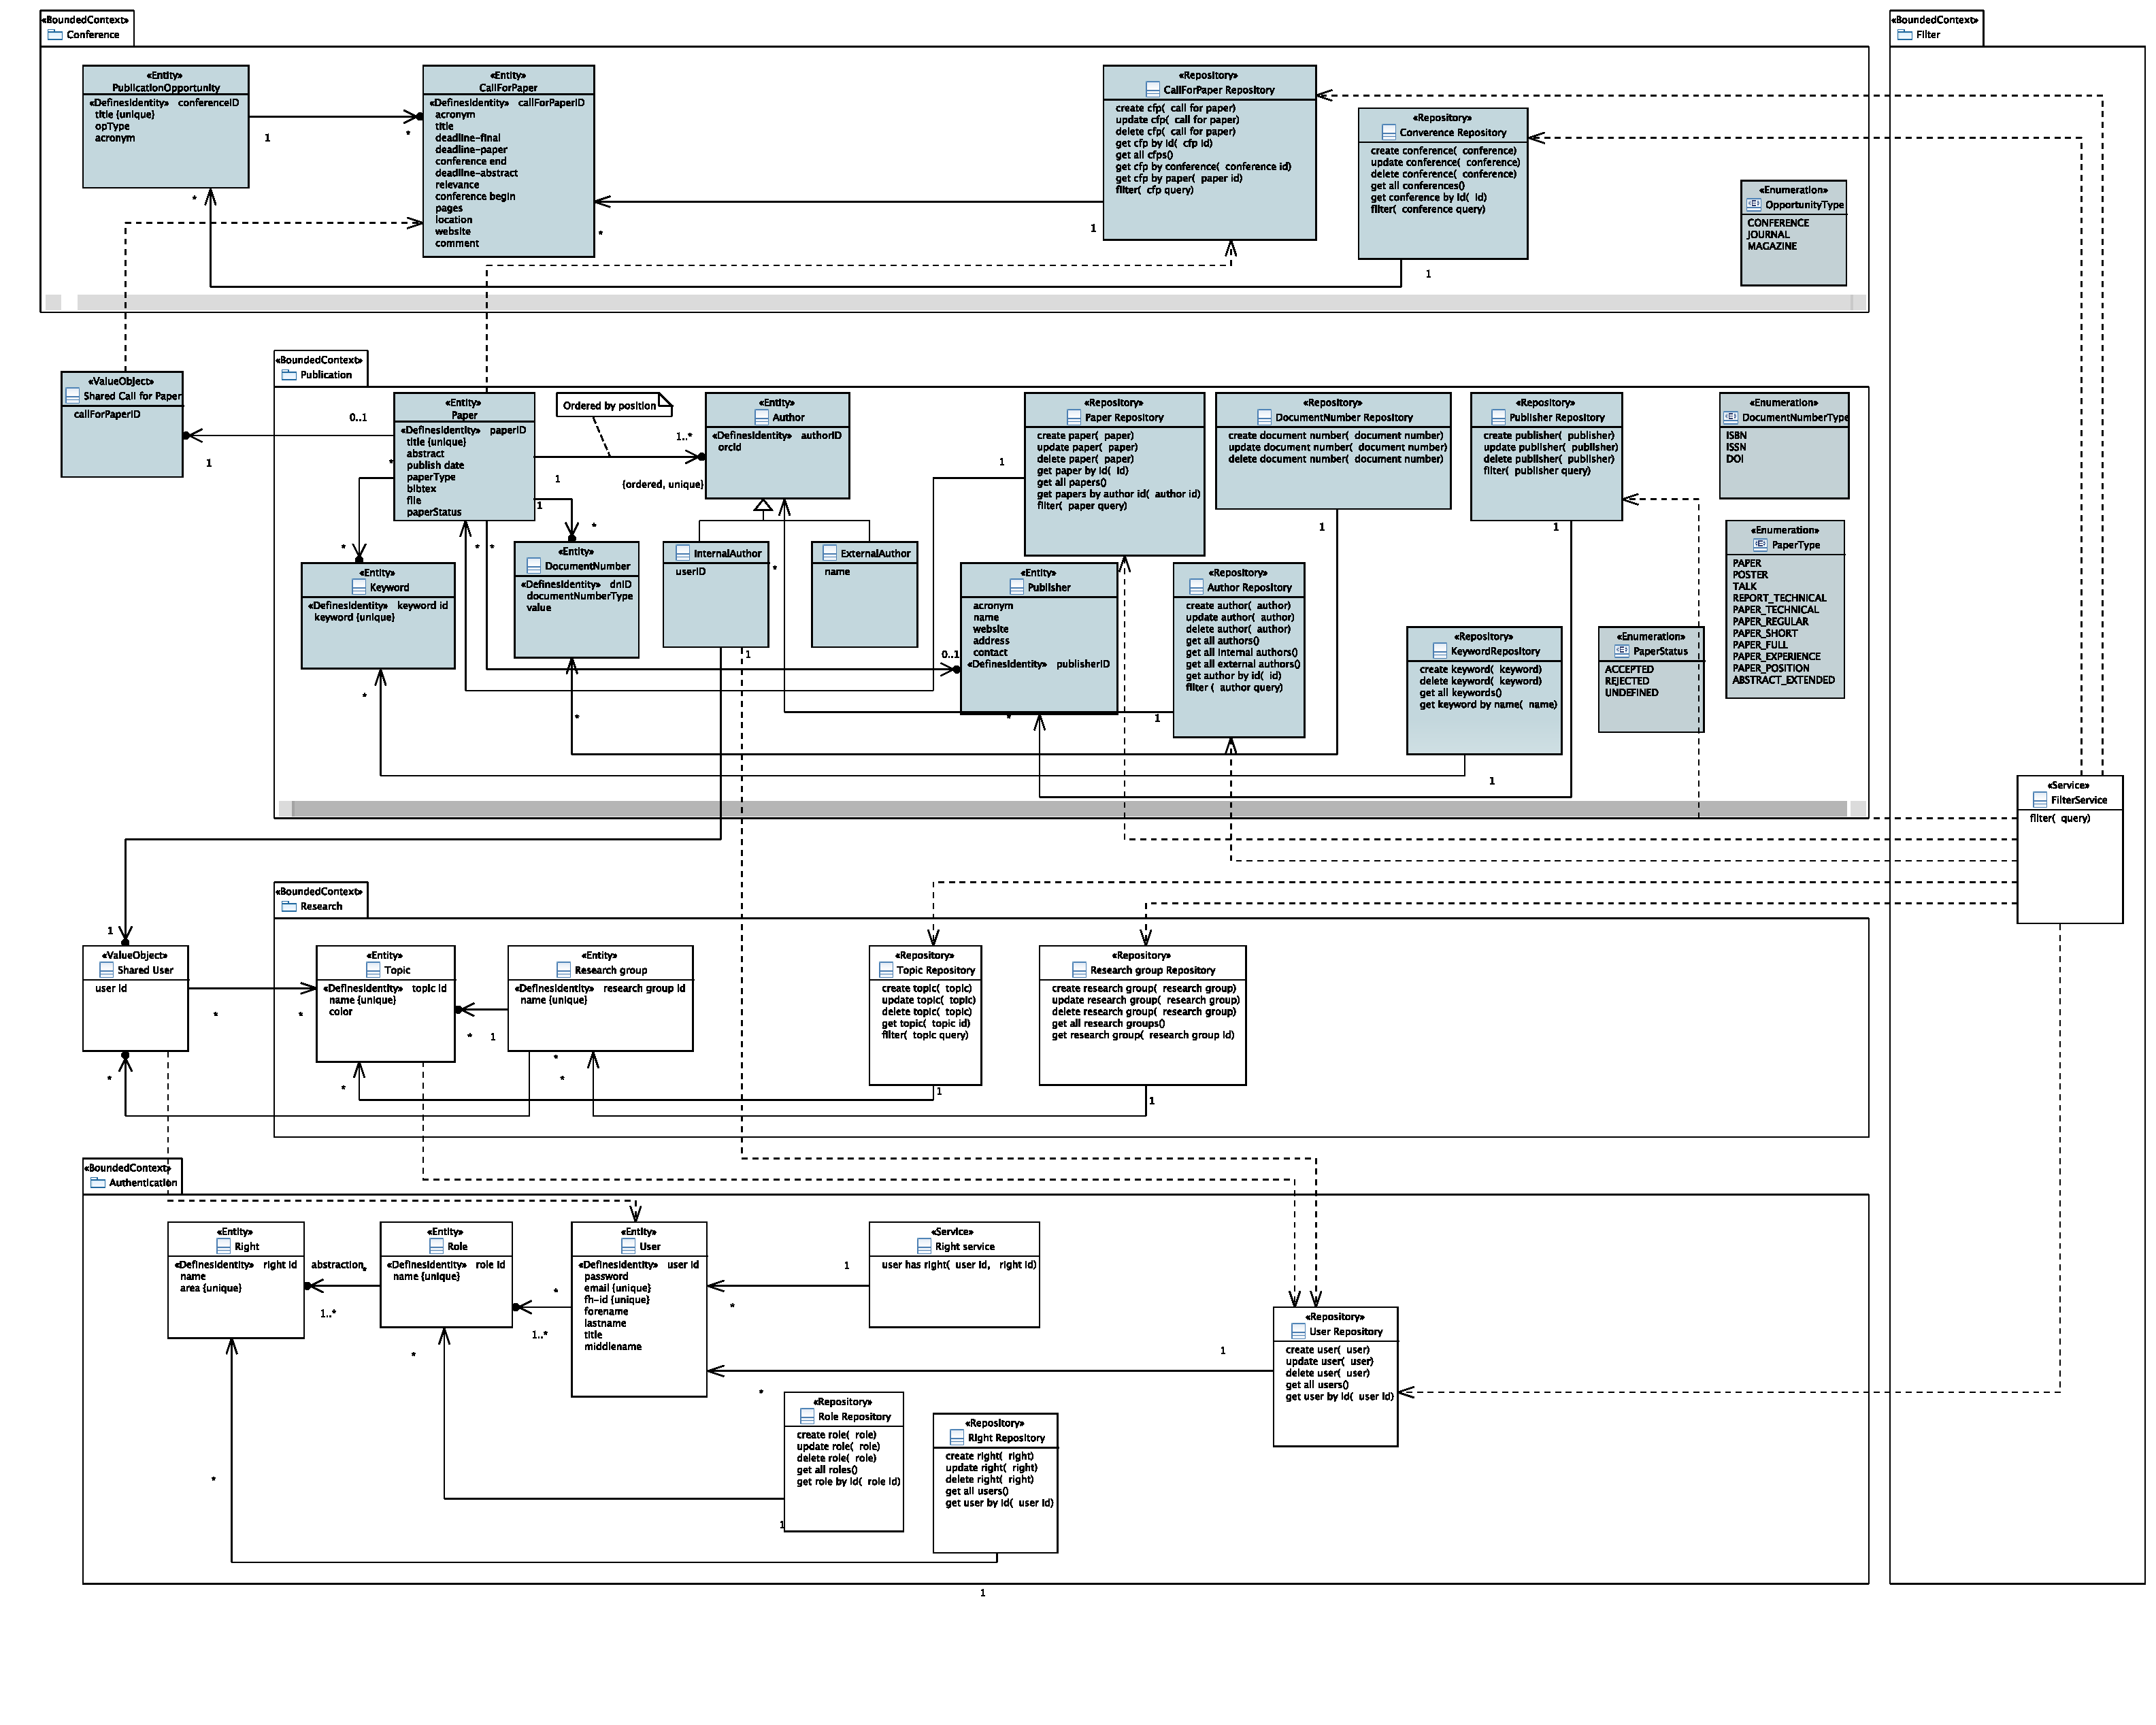
\includegraphics[width=\textwidth]{Bilder/rms_diagram.pdf}
\caption{Research Management System als UML Modell}
\end{figure}
\chapter{Abschluss}
\label{chap:zusammenfassung}
\section{Zusammenfassung}
\section{Fazit}
Anregung von Änderungen in ajil (Änderbarkeit von source und dataModel + Komplexe Datentypen für Entitäten.)
\section{Ausblick}
Ausführlichere null Checks und Überarbeitung des Moduls mit OCL erfahrenem Entwickler, da Autor dieser Arbeit nur rudimentäre OCL Kenntnisse besitzt

Weitere Anpassungen an \ac{ajil} können akkuratere Transformation ermöglichen (z.B. mehrere DataModels)
	

% Abkürzungsverzeichnis ins Inhaltsverzeichnis aufnehmen und mit Inhalt füllen
\cleardoublepage\phantomsection\addcontentsline{toc}{chapter}{Abkürzungsverzeichnis}
\chapter*{Abkürzungsverzeichnis}
	\begin{acronym}[NMWC] % längste Abkürzung steht in eckigen Klammern
    	\setlength{\itemsep}{-\parsep} % geringerer Zeilenabstand
    	\acro{ajil}[AjiL]{\textit{Ajil Modeling Language}}
    	\acro{atl}[ATL]{\textit{Atlas Transformation Language}}
		\acro{ddd}[DDD] {\textit{Domain-driven Design}}
		\acro{dsl}[DSL]{\textit{Domain Specific Language}}
		\acro{dsml}[DSML]{\textit{Domain Specific Modelling Language}}
		\acro{edm}[EDM]{\textit{Example-driven Modelling}}
		\acro{emp}[EMP]{\textit{Eclipse Modeling Project}}
		\acro{emf}[EMF]{\textit{Eclipse Modeling Framework}}
		\acro{emftvm}[EMFTVM]{\textit{EMF Transformation Virtual Machine}}
		\acro{gpl}[GPL]{\textit{General Purpose Language}}
		\acro{idial}[IDiAL]{\textit{Institut für die Digitalisierung von Arbeits- und Lebenswelten}}
		\acro{ide} [IDE] {\textit{Integrated Development Environment}}
		\acro{mdsd}[MDSD]{\textit{Model Driven Software Development}}
		\acro{m2m}[M2M]{\textit{Model To Model}}
		\acro{m2t}[M2T]{\textit{Model To Text}}
		\acro{mof}[MOF]{\textit{Meta Object Facility}}
		\acro{msa}[MSA]{\textit{Microservice Architecture}}
		\acro{omg}[OMG]{\textit{Object Management group}}
		\acro{ocl}[OCL]{\textit{Object Constraint Language}}
		\acro{rest}[REST]{\textit{Representational State Transfer }}
		\acro{soa}[SOA]{\textit{Service Oriented Architecture}}
		\acro{sus}[SuS]{\textit{System Under Study}}
		\acro{uml}[UML] {\textit{Unified Modeling Language}}
		\acro{qvt}[QVT]{\textit{Query/View/Transformation}}
\end{acronym}

\newpage{}

% Weitere Verzeichnisse ins Inhaltsverzeichnis aufnehmen
\cleardoublepage\phantomsection\addcontentsline{toc}{chapter}{Abbildungsverzeichnis}
\listoffigures

\newpage{}

\cleardoublepage\phantomsection\addcontentsline{toc}{chapter}{Tabellenverzeichnis}
\listoftables

\lstlistoflistings 
	
% Literaturverzeichnis setzen
\bibliographystyle{alphadin}
\bibliography{bib}
	
% Eidesstattliche Erklärung. ACHTUNG: Korrekten Text bitte unbedingt vorab mit Studienbüro klären!
\chapter*{Eidesstattliche Erklärung}
\thispagestyle{empty}
\textbf{ACHTUNG: Korrekten Text bitte unbedingt vorab mit Studienbüro klären!}\\
Hiermit versichere ich gemäß § 18 Abs. 5 der Bachelor-Prüfungsordnung des Studiengangs Informatik aus dem Jahr 2013, dass ich die  vorliegende Arbeit selbstständig angefertigt und mich keiner fremden Hilfe bedient, sowie keine anderen als die angegebenen Quellen und Hilfsmittel benutzt habe. Alle Stellen, die wörtlich oder sinngemäß veröffentlichten oder nicht veröffentlichten Schriften und anderen Quellen entnommen sind, habe ich als solche kenntlich gemacht. Diese Arbeit hat in gleicher oder ähnlicher Form noch keiner Prüfungsbehörde vorgelegen.

\vspace{1\baselineskip}%
Dortmund, \fhdopaperdate \hfill \fhdopaperauthor
\end{document}